\section{SSLStrip+}

%%%%%%%%%%%%%%%%%%%%%%%%%%%%%%%%%%%%
% HSTS                             %
%%%%%%%%%%%%%%%%%%%%%%%%%%%%%%%%%%%%
\begin{frame}{Fonctionnement de HSTS}
  \begin{columns}
    \begin{column}{0.6\textwidth}
      \begin{exampleblock}{HTTP Strict Transport Security}
        \begin{itemize}
        \item RFC 6797
        \item Entête HTTP 'Strict-Transport-Security'
        \item Date d'expiration
        \end{itemize}
      \end{exampleblock}

      \begin{alertblock}{Problème}
        \begin{itemize}
        \item Ne protège pas la première connexion
        \end{itemize}
      \end{alertblock}

      \begin{block}{Solution}
        \begin{itemize}
        \item HSTS preload
        \end{itemize}
      \end{block}

    \end{column}
    \begin{column}{0.4\textwidth}
      \begin{figure}
        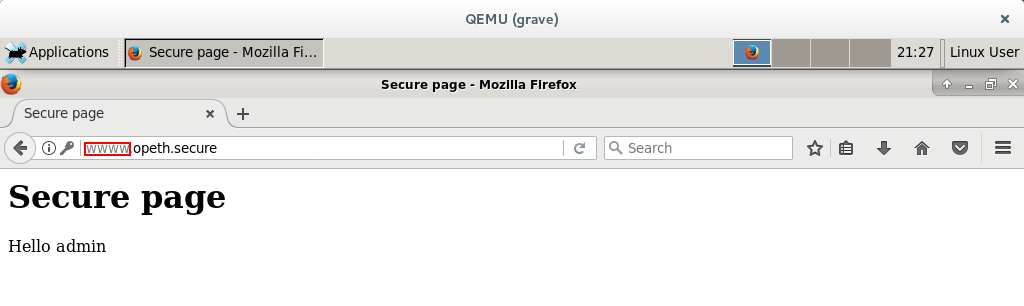
\includegraphics[width=\linewidth]{../medias/sslstrip2/screen2.png}
      \end{figure}
      \begin{figure}
        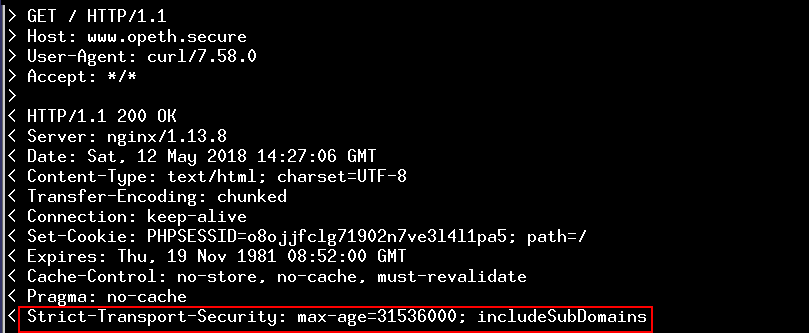
\includegraphics[width=\linewidth]{../medias/hsts.png}
      \end{figure}
    \end{column}
  \end{columns}

\end{frame}

%%%%%%%%%%%%%%%%%%%%%%%%%%%%%%%%%%%%
% SSLstrip+                        %
%%%%%%%%%%%%%%%%%%%%%%%%%%%%%%%%%%%%

\begin{frame}[fragile]{Attaque SSLStrip+}
  \begin{block}{Principes}
    \begin{itemize}
    \item{Attaquer le trafic DNS}
    \item{Utiliser un faux nom de domaine}
    \item{Remplacer les URL sécurisées par le faux nom}
    \end{itemize}
  \end{block}

  \begin{figure}
    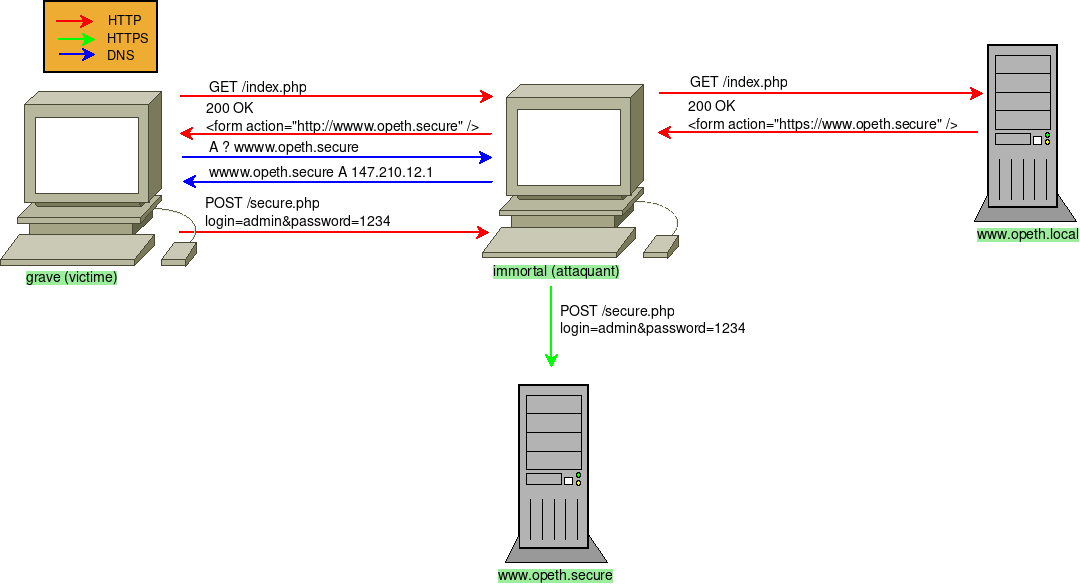
\includegraphics[width=0.86\linewidth]{../medias/sslstrip2/attack.png}
  \end{figure}
\end{frame}

\begin{frame}{Attaque SSLStrip+}
  \begin{figure}
    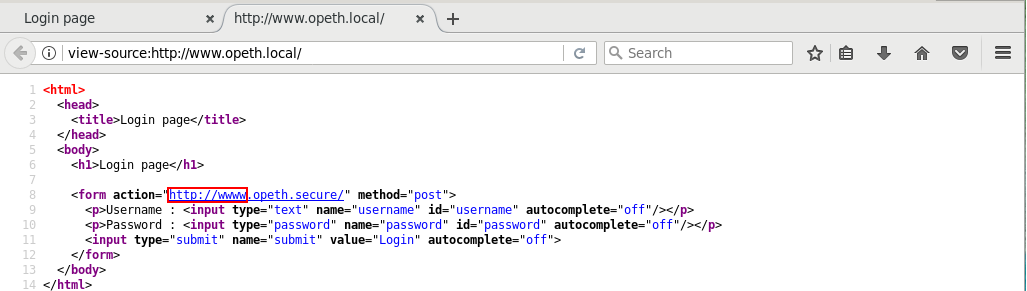
\includegraphics[width=1.0\linewidth]{../medias/sslstrip2/screen5-2.png}
  \end{figure}

  \begin{figure}
    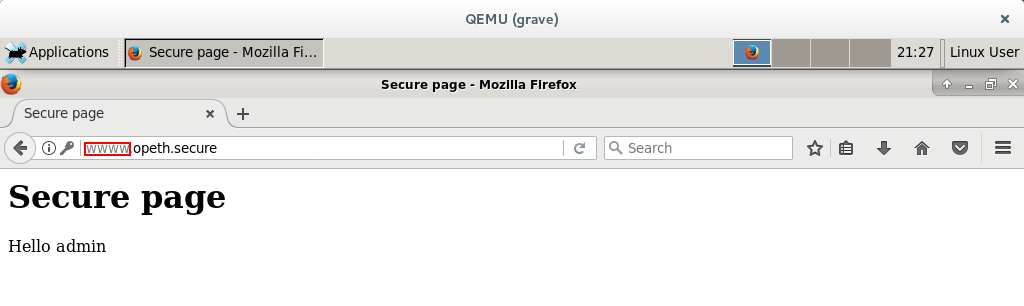
\includegraphics[width=1.0\linewidth]{../medias/sslstrip2/screen6.png}
  \end{figure}

\end{frame}
